% !TEX root = ../main.tex

% Exercises section

\section{Supplementary Plots}

\begin{table}[H]
\centering
\begin{tabular}{|l|l|l|l|}
\hline
& treatment & & gender\\
\hline
intervention & 0.576 & male & 0.341 \\
\hline
control & 0.424 & female & 0.659\\
\hline
\end{tabular}
\caption{Summary statistics (proportion) for categorical variables}
\label{tab:summ.stat.cat}
\end{table}

\begin{table}[H]
\centering
\begin{tabular}{|l|l|l|l|l|}
\hline
& month & month + gender & month + education & month + gender + education \\
\hline
AIC & 2756.056 & 2731.897 & 2717.689 & 2705.601 \\
\hline
BIC & 2768.067 & 2747.902 & 2733.695 & 2725.595 \\
\hline
\end{tabular}
\caption{Comparison of models with different covariates under the control group}
\label{tab:model.comp.control}
\end{table}

\begin{table}[H]
\centering
\begin{tabular}{|l|l|l|l|}
\hline
& month & month + gender & month + education \\
\hline
intervention & 0.016 & 0 & 0 \\
\hline
control & 0 & 0 & 0 \\
\hline
\end{tabular}
\caption{P values of Likelihood Ratio tests between models with different covariates for each treatment group}
\label{tab:model.comp.sep.lrt}
\end{table}

\begin{figure}[H]
\begin{subfigure}{.33\textwidth}
  \centering
  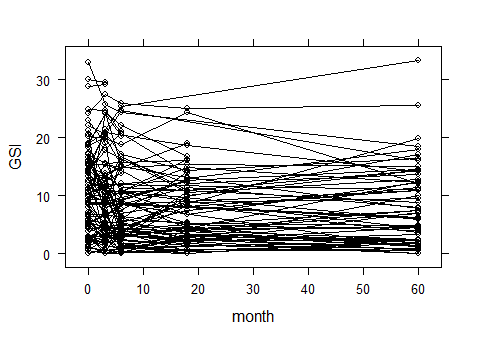
\includegraphics[width=1\linewidth]{../../plots/trellis_control.png}
  \caption{trellis plot of all subjects in the control group}
\end{subfigure}
\begin{subfigure}{.33\textwidth}
  \centering
  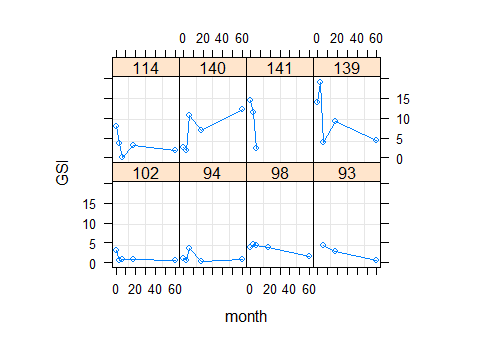
\includegraphics[width=1\linewidth]{../../plots/trellis_subset_control.png}
  \caption{trellis plot of randomly selected subjects}
\end{subfigure}
\begin{subfigure}{.33\textwidth}
  \centering
  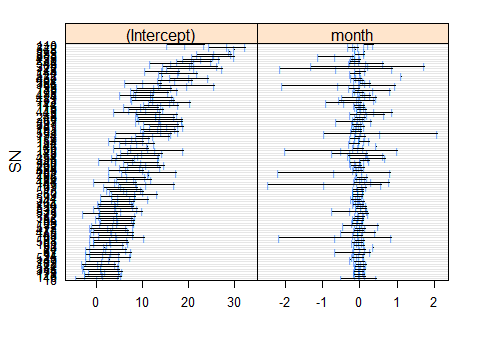
\includegraphics[width=1\linewidth]{../../plots/interval_control.png}
  \caption{confidence intervals of parameters from individual linear models}
\end{subfigure}
\caption{Diagnostic plots for selection of random effects for the control group}
\label{fig:diagnostic.control}
\end{figure}

\begin{table}[H]
\centering
\begin{tabular}{|l|l|l|l|}
\hline
& no mixed effect & mixed effect on intercept & mixed effect on both intercept and month \\
\hline
AIC & 2705.601 & 2415.440 & 2415.845 \\
\hline
BIC & 2725.595 & 2439.433 & 2447.837 \\
\hline
\end{tabular}
\caption{Comparison of models with different mixed effects under the control group}
\label{tab:model.comp.control.me}
\end{table}

\begin{table}[H]
\centering
\resizebox{\linewidth}{!}{
\begin{tabular}{|l|l|l|l|}
\hline
& no mixed effect & mixed effect on intercept & mixed effect on both intercept and month \\
\hline
no mixed effect & N/A & 0 & 0 \\
\hline
mixed effect on intercept & 0 & N/A & 0.166 \\
\hline
mixed effect on both intercept and month & 0 & 0.166 & N/A \\
\hline
\end{tabular}
}
\caption{P values of Likelihood Ratio tests between models with different mixed effects under the control group}
\label{tab:model.comp.control.me.lrt}
\end{table}

\begin{table}[H]
\centering
\begin{tabular}{|l|l|l|l|l|}
\hline
& month & month + gender & month + education & month + gender + education \\
\hline
AIC & 6733.685 & 6676.801 & 6695.365 & 6650.988 \\
\hline
BIC & 6753.371 & 6701.404 & 6719.968 & 6680.506 \\
\hline
\end{tabular}
\caption{Comparison of models with different covariates}
\label{tab:model.comp}
\end{table}

\begin{table}[H]
\centering
\begin{tabular}{|l|l|l|}
\hline
month & month + gender & month + education \\
\hline
0 & 0 & 0 \\
\hline
\end{tabular}
\caption{P values of Likelihood Ratio tests between models with different covariates}
\label{tab:model.comp.lrt}
\end{table}

\begin{table}[H]
\centering
\begin{tabular}{|l|l|l|l|}
\hline
& no mixed effect & mixed effect on intercept & mixed effect on both intercept and month \\
\hline
AIC & 6650.988 & 6060.302 & 6053.840 \\
\hline
BIC & 6680.506 & 6094.740 & 6098.118 \\
\hline
\end{tabular}
\caption{Comparison of models with different mixed effects}
\label{tab:model.comp.me}
\end{table}

\begin{table}[H]
\centering
\resizebox{\linewidth}{!}{
\begin{tabular}{|l|l|l|l|}
\hline
& no mixed effect & mixed effect on intercept & mixed effect on both intercept and month \\
\hline
no mixed effect & N/A & 0 & 0 \\
\hline
mixed effect on intercept & 0 & N/A & 0.005 \\
\hline
mixed effect on both intercept and month & 0 & 0.005 & N/A \\
\hline
\end{tabular}
}
\caption{P values of Likelihood Ratio tests between models with different mixed effects}
\label{tab:model.comp.me.lrt}
\end{table}

\begin{table}[H]
\centering
\begin{tabular}{|l|r|r|r|r|r|}
\hline
  & Value & Std.Error & DF & t-value & p-value\\
\hline
(Intercept) & 19.235 & 4.151 & 308 & 4.634 & 0.000\\
\hline
month & -0.020 & 0.008 & 308 & -2.394 & 0.017\\
\hline
gender2 & 2.606 & 1.383 & 95 & 1.884 & 0.063\\
\hline
education & -0.822 & 0.273 & 95 & -3.015 & 0.003\\
\hline
\end{tabular}
\caption{Output of Linear Mixed Model under the control group}
\label{tab:lme.control}
\end{table}

\begin{figure}[H]
\begin{subfigure}{.5\textwidth}
  \centering
  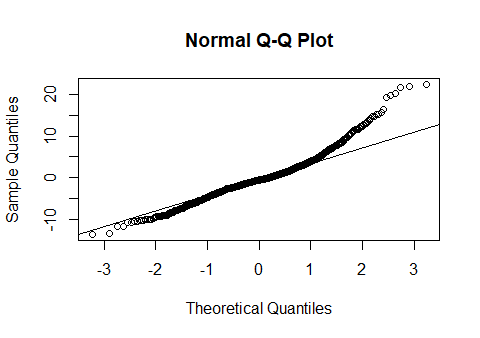
\includegraphics[width=1\linewidth]{../../plots/qq_residual_control.png}
  \caption{residual QQ plot}
\end{subfigure}
\begin{subfigure}{.5\textwidth}
  \centering
  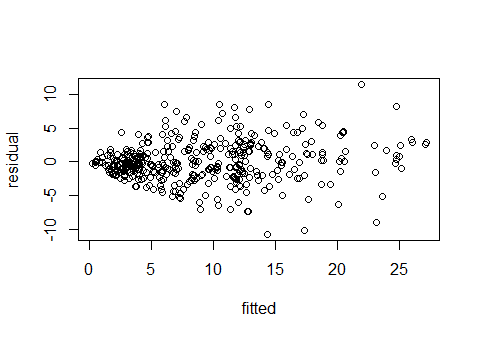
\includegraphics[width=1\linewidth]{../../plots/residual_control.png}
  \caption{fitted value vs. residual (t-test: 1, Wilcoxon: 0.501)}
\end{subfigure}
\caption{Visualizing the residuals of the LME model under the control group}
\label{fig:residual.control}
\end{figure}

\begin{figure}[H]
\centering
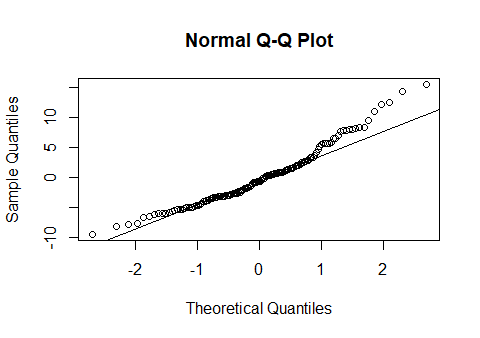
\includegraphics[width=0.5\linewidth]{../../plots/qq_intercept_treatment.png}
\caption{QQ plot for the random effects on the intercept (t-test: 1, Wilcoxon: 0.405)}
\label{fig:re.control}
\end{figure}

\begin{table}[H]
\centering
\begin{tabular}{|l|r|r|r|r|r|}
\hline
  & Estimate & Naive S.E. & Naive z & Robust S.E. & Robust z\\
\hline
(Intercept) & 19.267 & 3.433 & 5.613 & 3.229 & 5.967\\
\hline
month & -0.027 & 0.013 & -2.019 & 0.010 & -2.606\\
\hline
gender2 & 2.220 & 1.148 & 1.935 & 1.216 & 1.825\\
\hline
education & -0.809 & 0.225 & -3.596 & 0.203 & -3.994\\
\hline
\end{tabular}
\caption{Output of GEE model under the control group}
\label{tab:gee.control}
\end{table}

\begin{table}[H]
\centering
\begin{tabular}{|l|r|r|r|r|r|}
\hline
  & Value & Std.Error & DF & t-value & p-value\\
\hline
(Intercept) & 15.418 & 2.341 & 774 & 6.586 & 0.000\\
\hline
treatment2 & -0.193 & 0.731 & 238 & -0.264 & 0.792\\
\hline
month & -0.037 & 0.006 & 774 & -5.893 & 0.000\\
\hline
gender2 & 2.737 & 0.776 & 238 & 3.527 & 0.001\\
\hline
education & -0.516 & 0.157 & 238 & -3.295 & 0.001\\
\hline
\end{tabular}
\caption{Output of Linear Mixed Model}
\label{tab:lme}
\end{table}

\begin{figure}[H]
\begin{subfigure}{.5\textwidth}
  \centering
  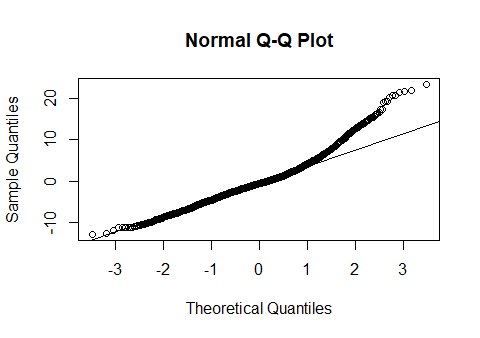
\includegraphics[width=1\linewidth]{../../plots/qq_residual.png}
  \caption{residual QQ plot}
\end{subfigure}
\begin{subfigure}{.5\textwidth}
  \centering
  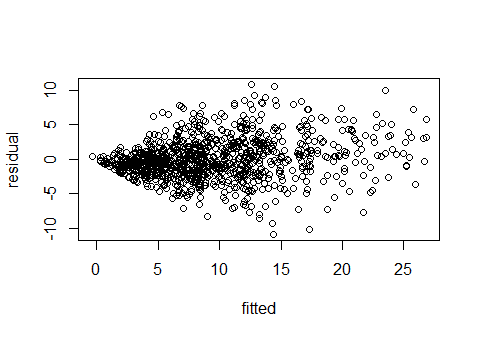
\includegraphics[width=1\linewidth]{../../plots/residual.png}
  \caption{fitted value vs. residual (t-test: 1, Wilcoxon: 0.143)}
\end{subfigure}
\caption{Visualizing the residuals of the LME model}
\label{fig:residual}
\end{figure}

\begin{figure}[H]
\begin{subfigure}{.5\textwidth}
  \centering
  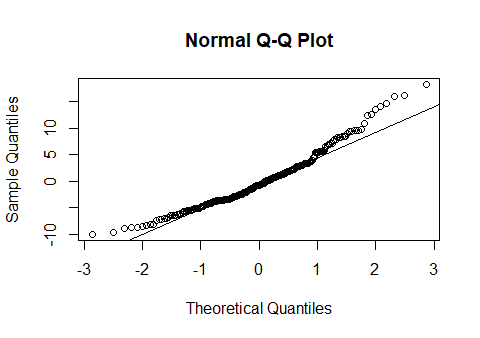
\includegraphics[width=1\linewidth]{../../plots/qq_intercept.png}
  \caption{QQ plot for the random effects on the intercept (t-test: 1, Wilcoxon: 0.207)}
\end{subfigure}
\begin{subfigure}{.5\textwidth}
  \centering
  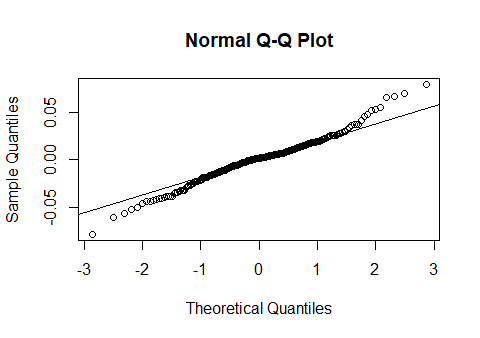
\includegraphics[width=1\linewidth]{../../plots/qq_slope.png}
  \caption{QQ plot for the random effects on the slope (t-test: 1, Wilcoxon: 0.786)}
\end{subfigure}
\caption{Visualizing the random effects}
\label{fig:re}
\end{figure}

\begin{table}[H]
\centering
\begin{tabular}{|l|r|r|r|r|r|}
\hline
  & Estimate & Naive S.E. & Naive z & Robust S.E. & Robust z\\
\hline
(Intercept) & 14.685 & 2.046 & 7.176 & 2.053 & 7.154\\
\hline
treatment2 & -0.430 & 0.641 & -0.671 & 0.735 & -0.586\\
\hline
month & -0.039 & 0.008 & -4.666 & 0.006 & -6.040\\
\hline
gender2 & 2.693 & 0.680 & 3.961 & 0.716 & 3.763\\
\hline
education & -0.455 & 0.136 & -3.337 & 0.139 & -3.278\\
\hline
\end{tabular}
\caption{Output of GEE model}
\label{tab:gee}
\end{table}

\begin{table}[H]
\centering
\begin{tabular}{|l|r|r|r|r|r|r|r|}
\hline
  & Estimate & Std.Error & t.value & df & P value & RIV & FMI\\
\hline
(Intercept) & 11.526 & 2.809 & 4.104 & 231.840 & 0.000 & 0.151 & 0.139\\
\hline
month & -0.045 & 0.011 & -3.999 & 23.557 & 0.001 & 0.701 & 0.456\\
\hline
gender2 & 2.734 & 0.968 & 2.824 & 239.207 & 0.005 & 0.149 & 0.137\\
\hline
education & -0.222 & 0.199 & -1.115 & 107.937 & 0.268 & 0.238 & 0.207\\
\hline
\end{tabular}
\caption{Output of pooled Linear Mixed Model under the intervention group}
\label{tab:lme.treatment.mi}
\end{table}

\begin{table}[H]
\centering
\begin{tabular}{|l|r|r|r|r|r|r|r|}
\hline
  & Estimate & Std.Error & t.value & df & P value & RIV & FMI\\
\hline
(Intercept) & 19.695 & 4.011 & 4.910 & 1786.900 & 0.000 & 0.050 & 0.048\\
\hline
month & -0.032 & 0.012 & -2.571 & 10.407 & 0.027 & 1.631 & 0.677\\
\hline
gender2 & 2.277 & 1.315 & 1.732 & 5112.727 & 0.083 & 0.029 & 0.028\\
\hline
education & -0.828 & 0.268 & -3.096 & 802.808 & 0.002 & 0.076 & 0.073\\
\hline
\end{tabular}
\caption{Output of pooled Linear Mixed Model under the control group}
\label{tab:lme.control.mi}
\end{table}

\begin{table}[H]
\centering
\begin{tabular}{|l|r|r|r|r|r|r|r|}
\hline
  & Estimate & Std.Error & t.value & df & P value & RIV & FMI\\
\hline
(Intercept) & 11.102 & 2.789 & 3.981 & 158.677 & 0.000 & 0.189 & 0.169\\
\hline
month & -0.048 & 0.012 & -4.090 & 12.698 & 0.001 & 1.279 & 0.617\\
\hline
gender2 & 2.733 & 0.942 & 2.902 & 355.509 & 0.004 & 0.119 & 0.111\\
\hline
education & -0.188 & 0.198 & -0.947 & 78.666 & 0.347 & 0.291 & 0.244\\
\hline
\end{tabular}
\caption{Output of pooled GEE model (naive) under the intervention group}
\label{tab:gee.treatment.mi.naive}
\end{table}

\begin{table}[H]
\centering
\begin{tabular}{|l|r|r|r|r|r|r|r|}
\hline
  & Estimate & Std.Error & t.value & df & P value & RIV & FMI\\
\hline
(Intercept) & 20.598 & 4.119 & 5.000 & 208.709 & 0.000 & 0.161 & 0.147\\
\hline
month & -0.027 & 0.014 & -1.999 & 14.750 & 0.064 & 1.087 & 0.575\\
\hline
gender2 & 1.821 & 1.328 & 1.371 & 440.506 & 0.171 & 0.105 & 0.099\\
\hline
education & -0.870 & 0.280 & -3.103 & 105.337 & 0.002 & 0.242 & 0.210\\
\hline
\end{tabular}
\caption{Output of pooled GEE model (naive) under the control group}
\label{tab:gee.control.mi.naive}
\end{table}

\begin{table}[H]
\centering
\begin{tabular}{|l|r|r|r|r|r|r|r|}
\hline
  & Estimate & Std.Error & t.value & df & P value & RIV & FMI\\
\hline
(Intercept) & 11.102 & 2.692 & 4.124 & 137.732 & 0.000 & 0.205 & 0.182\\
\hline
month & -0.048 & 0.012 & -3.939 & 14.758 & 0.001 & 1.086 & 0.575\\
\hline
gender2 & 2.733 & 0.908 & 3.009 & 307.277 & 0.003 & 0.129 & 0.120\\
\hline
education & -0.188 & 0.191 & -0.985 & 67.256 & 0.328 & 0.323 & 0.265\\
\hline
\end{tabular}
\caption{Output of pooled GEE model (robust) under the intervention group}
\label{tab:gee.treatment.mi.robust}
\end{table}

\begin{table}[H]
\centering
\begin{tabular}{|l|r|r|r|r|r|r|r|}
\hline
  & Estimate & Std.Error & t.value & df & P value & RIV & FMI\\
\hline
(Intercept) & 20.598 & 3.695 & 5.575 & 135.062 & 0.000 & 0.208 & 0.184\\
\hline
month & -0.027 & 0.014 & -1.949 & 16.329 & 0.069 & 0.980 & 0.547\\
\hline
gender2 & 1.821 & 1.302 & 1.399 & 406.382 & 0.163 & 0.110 & 0.104\\
\hline
education & -0.870 & 0.242 & -3.590 & 58.813 & 0.001 & 0.353 & 0.285\\
\hline
\end{tabular}
\caption{Output of pooled GEE model (robust) under the control group}
\label{tab:gee.control.mi.robust}
\end{table}

\begin{table}[H]
\centering
\begin{tabular}{|l|r|r|r|r|r|r|r|}
\hline
  & Estimate & Std.Error & t.value & df & P value & RIV & FMI\\
\hline
(Intercept) & 14.858 & 2.439 & 6.091 & 135.244 & 0.000 & 0.208 & 0.184\\
\hline
treatment2 & -0.171 & 0.733 & -0.234 & 802.931 & 0.815 & 0.076 & 0.073\\
\hline
month & -0.039 & 0.009 & -4.167 & 15.060 & 0.001 & 1.063 & 0.569\\
\hline
gender2 & 2.604 & 0.829 & 3.139 & 108.962 & 0.002 & 0.237 & 0.206\\
\hline
education & -0.467 & 0.172 & -2.715 & 58.348 & 0.009 & 0.355 & 0.286\\
\hline
\end{tabular}
\caption{Output of pooled Linear Mixed Model}
\label{tab:lme.mi}
\end{table}

\begin{table}[H]
\centering
\begin{tabular}{|l|r|r|r|r|r|r|r|}
\hline
  & Estimate & Std.Error & t.value & df & P value & RIV & FMI\\
\hline
(Intercept) & 14.644 & 2.449 & 5.980 & 98.809 & 0.000 & 0.252 & 0.217\\
\hline
treatment2 & -0.223 & 0.724 & -0.307 & 832.892 & 0.759 & 0.074 & 0.072\\
\hline
month & -0.039 & 0.011 & -3.678 & 8.707 & 0.005 & 2.104 & 0.733\\
\hline
gender2 & 2.591 & 0.810 & 3.197 & 140.824 & 0.002 & 0.203 & 0.180\\
\hline
education & -0.446 & 0.173 & -2.582 & 48.524 & 0.013 & 0.403 & 0.315\\
\hline
\end{tabular}
\caption{Output of pooled GEE model (naive)}
\label{tab:gee.mi.naive}
\end{table}

\begin{table}[H]
\centering
\begin{tabular}{|l|r|r|r|r|r|r|r|}
\hline
  & Estimate & Std.Error & t.value & df & P value & RIV & FMI\\
\hline
(Intercept) & 14.644 & 2.356 & 6.215 & 84.692 & 0.000 & 0.278 & 0.235\\
\hline
treatment2 & -0.223 & 0.742 & -0.300 & 917.614 & 0.764 & 0.071 & 0.068\\
\hline
month & -0.039 & 0.011 & -3.594 & 9.554 & 0.005 & 1.833 & 0.703\\
\hline
gender2 & 2.591 & 0.786 & 3.298 & 124.401 & 0.001 & 0.218 & 0.192\\
\hline
education & -0.446 & 0.168 & -2.655 & 43.400 & 0.011 & 0.436 & 0.334\\
\hline
\end{tabular}
\caption{Output of pooled GEE model (robust)}
\label{tab:gee.mi.robust}
\end{table}